% !TEX root = Report.tex


\newpage
\section{Test Case Simulation Plots and Commentary}
In this section, we include the plots resulting from our simulation running
on various testcases. 

\subsection{TCP Vegas}
For TCP Vegas, we see, more or less, the expected behavior on each of the test
cases.

\subsubsection{Test Case 0}
We only have one link to analyze, and we see that
the rate across this link goes through a brief period of slow start at the
beginning, fluctuates for a little bit as it converges, and then
stays relatively constant at 10 Mbps. This accurately reflects
Vegas behavior, which goes through slow start and then should stabilize as the
diff parameter (cwnd * (1/rttmin - 1/rttcurrent)) gets between alpha and beta.
As for the actual value, we see that it stabilizes to something like 10.6 Mbps.
This makes sense because of the way our network is set up. Our links are
implemented such that it has a buffer on each side (for each direction). Each
buffer has the capacity that the link should have. So, the theoretical maximum
of our link rates is actually 2 times the specified rate. The 10.6 Mbps rate
on link one makes sense because the algorithm will stabilize naturally to send
data across the link at the capacity. So, it will send data packets from 
host 1 to host 2 at 10 Mbps. The other 0.6 Mbps is a result of the ack packets
being returned in the other direction. Because ack packets are about 6\%
the size of data packets (64 vs 1024 bytes) this result makes sense.

The buffer occupancy graph oscillates between two values. This happens even
with a constant window size because the host will send out its window size
(which corresponds to the higher buffer occupancy), and then wait until it
receives acknowledgements. In that time, the buffer occupancy is slightly lower.

The packet loss of this test case is 0 because no packets are ever lost,
fast-retransmit occurs first. There are no other flows, so there is not enough
congestion to actually lose packets.

The flow send rate, window size, and packet delay all behave as expected,
with a slow start rise, followed by minor fluctuations during the convergence,
and finishing with a stable value. The flow rate of 10 Mbps is as expected,
because that is the bottleneck link's rate.

\subsubsection{Test Case 1}
The link rates behave pretty similarly to test cae 0, except with an
oscillating behavior. During the first 5 seconds, the routing table shows the
same weights for both paths through the network because there is no congestion.
So, the flow goes through the same slow start an convergence pattern, and then
stabilizes to about 10 Mbps from host 1 to host 2 and 0.6 Mbps in the opposite
direction.
Our network is implemented that it finds any path with the min weight and
forwards packets along that. It happens that on the way from host 1 to host 2,
the data packets are forwarded along link 2 at 10 Mbps, which is the expected
rate. On the return path, the ack packets are forwarded along link 1 (the
choice is arbitrary). So, there is about 0.6 Mbps activity on link 1, similar
to test case 0. After the next routing table update, the links behave in
an oscillating pattern. After 5 seconds, the lower path is more congested,
so the tables change to reflect this and forward all packets along the upper
path, resulting in 10.6 Mbps activity along link 1. After this, the upper
path is more congested and the routing tables change to forward packets
along the lower path, and so on until completion.

The buffer occupancy graphs show that the link with the congestion has
a growing buffer occupancy from the beginning of the period
(separated by routing table updates) and then stabilizes for the rest of the
period. The growing behavior is due to the routing table updates. The paths
the packets follow is changed, so there is some time as the packets go through
the link and gradually fill the buffer until they reach the stablized value.

Again, packet loss is 0 throughout the duration of the simulation because no
packets are lost, retransmits only happen as result of duplicate
acknowledgements.

Flow rate, window size, and packet delay all follow the behavior seen in
link rate and buffer occupancy.
This, of course, makes sense as they are all related. The flow
rate of 10 Mbps also reflects the expected behavior of Vegas.

\subsubsection{Test Case 2}
The analysis of test case 2 with Vegas is done in the mathematical analysis
section.


\subsection{TCP Reno}
For TCP Reno, we see, more or less, the expected behavior on each of the test
cases.

\subsubsection{Test Case 0}
The link rate is again at the expected rate of 10.6 Mbps. It goes through the
same slow start rise at the beginning as Vegas, after which the behavior
is the same.

The buffer occupancy plots reflect the behavior of TCP Reno. They rise until
3 duplicate acknowledgements are received, at which point the window size is
set to 1, and so the buffer occupancy is similarly reduced. If a packet is lost,
the ssthresh is also changed, reflected in the decreasing bottoms of the rising
arcs.

The packet loss is 0 most of the time, but hits a few packet losses in the slow
start phase of Reno, as expected. After this, because it is a loss-based
congestion control, there are small blips of packet loss, which correspond
to the packet drops after the window gets sufficiently large.

The flow send rate, window size, and packet delay all behave as expected,
reflecting the behavior of the link rate and buffer occupancy.

\subsubsection{Test Case 1}
The link rate in test case 1 shows Reno's behavior in the oscillating
network. The link rates grow quickly in the beginning during slow start,
then it reaches the same state as Vegas, where the packets are first forwarded
along the bottom path (link 2) until the first routing table update, at which
point they switch to the other path, and back and forth. The rising behavior
of the rate is also expected, as it grows until it reaches the max of
about 10.6 Mbps (as before) before dropping, which is Reno's design.

The buffer occupancy behaves somewhat as expected. After slow start, it
stays quite low for a while, which is expected, and then starts growing
on one of the fork links between 10 and 15 seconds in. Similar behavior
occurs before 20 seconds, and before 25 seconds. This reflects the behavior of
links where the rates grow until they reach a max and get reduced.

The packet loss has some loss in the initial slow start phase, but no losses
afterward. This is expected because the routing table updates change the paths
of the packets, so none are actally dropped, but congestion control may happen
due to duplicate acks.

The flow send rate, window size, and packet delay all behave as expected,
reflecting the behavior of the link rate and buffer occupancy.

\subsubsection{Test Case 2}
The link rate in test case 2 shows Reno's behavior when there are mutiple
flows competing for resources.
The link rates grow quickly in the beginning during slow start,
and then the links all achieve rates of about 10.6 Mbps, because there is only
one flow going across all 3 links, so this is the expected behavior.
Once the second flow is added, the behavior changes. Because both flow 1 and
2 use link 1, that is still achieving its 10.6 Mbps rate. However, flow 1
continues on to use links 2 and 3. Because the bottleneck link 1 is
congested, the rates on those links are lower, as expected. With the addition
of the third flow, link 3 has the same behavior as link 1 because it is
essentially the same case. However, link 2 has the same behavior as before,
because only flow 1 is crossing it. As flow 2 ends, we see behavior similar
to when it was only flow 1 and 2, which makes sense because the simulation is
symmetric. When flow 2 ends, all the link flow rates increase back up to
the initial state, which is all links with rates of 10 Mbps.

The buffer occupancy behaves somewhat as expected. After slow start,
link 1 starts to fill because flow 1 sends it into the network and bottlenecks
at link 1, and the other 2 are unaffected. When the second flow joins, it is
the same kind of behavior, as we expect, because it is still just the one
bottleneck link. With the addition of the third flow, we expect occupancy
in buffers of links 1 and 3. We see that they overlap for a few seconds
(~25-30), where both the buffers are growing in size, as expected. As the
second flow ends, the buffer on link 1 drops in size, as expected. Because
flow 1 is forced to send at a lower rate due to the congestion at link 3, there
is also no buffer waiting at link 1, which is the behavior we see. After
flow 3 finishes, we see that it goes back to the initial behavior of link
1 growing in size.

The packet loss is as we expect. We see some losses during slow start, and
again when flow 3 joins, because there are too many packets entering the
system and some are dropped.

The packet delay shows the behavior we expect. We see that it starts with
rising delay for flow 1. As flow 2 is added in, they both grow, and flow 1
stays above it because while they have the same congestion on the outer links
and the shared link 1, flow 1 also has to go through links 2 and 3, which is
added delay. Similar behavior is seen with all 3 flows, though flow 3 has
lower delay than flow 2. This is because the queueing delay for flow 1 is
all in link 1, and there are fewer waiting packets in link 3, which allows
for flow 3 to achieve a lower delay. When flow 2 ends, we see similar behavior
as to when it was only flows 1 and 2, with flow 1 having longer delays due to
longer path.

The flow send rate and window size pretty much behave as expected,
reflecting the results seen in other stats.


%%%%%%%%%%%%%%%%%%%%%%%%%%%%%%%%%%%%%%%%%%%%%%%%%%%%%%%%%%%%%%%%%%%

\begin{figure}[htbp]
    \centering
    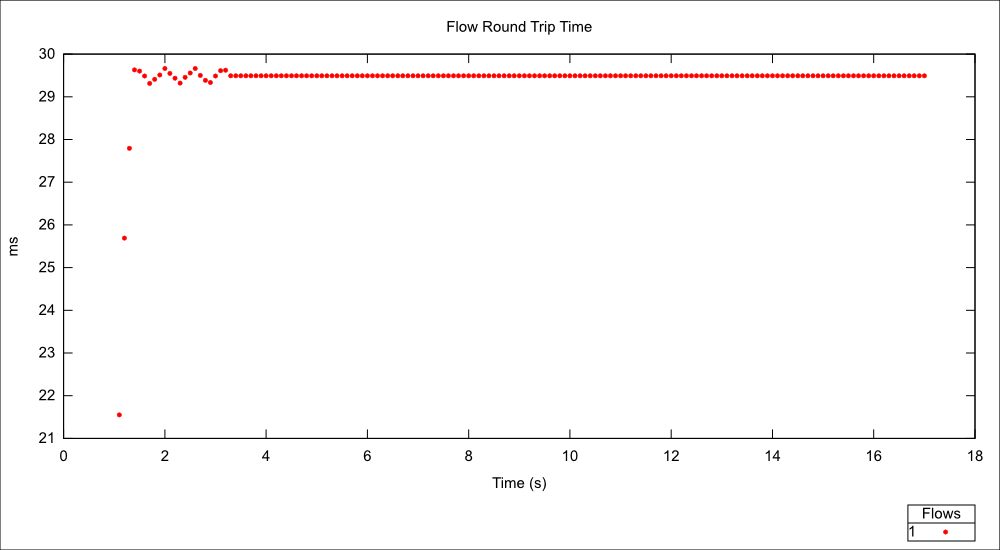
\includegraphics[width=\textwidth]{vegas0/Flow_RTT.png}
    \caption{TCP VEGAS, Case 0: Flow Round Trip Time}
\end{figure}

\begin{figure}[htbp]
    \centering
    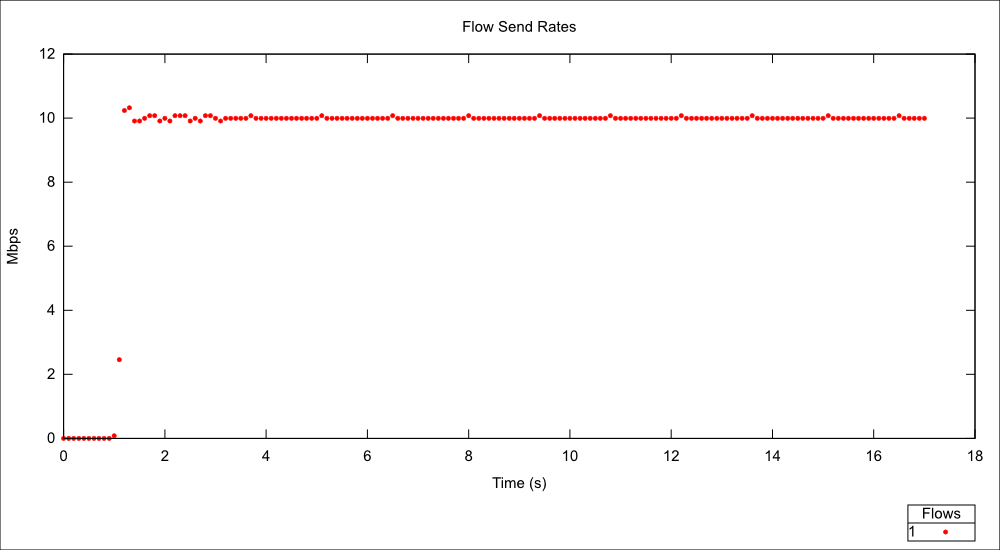
\includegraphics[width=\textwidth]{vegas0/Flow_Send_Rates.png}
    \caption{TCP VEGAS, Case 0: Flow Send Rates}
\end{figure}

\begin{figure}[htbp]
    \centering
    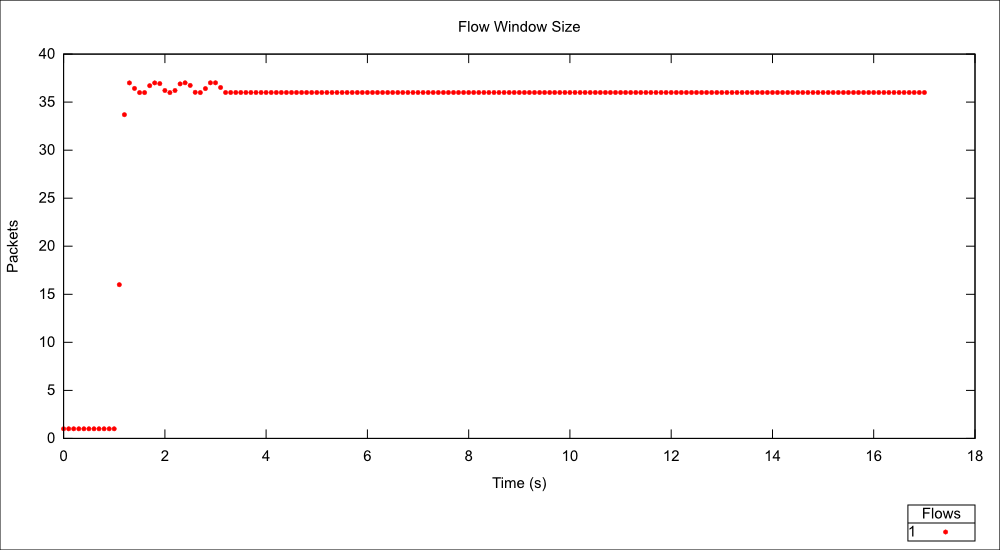
\includegraphics[width=\textwidth]{vegas0/Flow_Window.png}
    \caption{TCP VEGAS, Case 0: Flow Window}
\end{figure}


\begin{figure}[htbp]
    \centering
    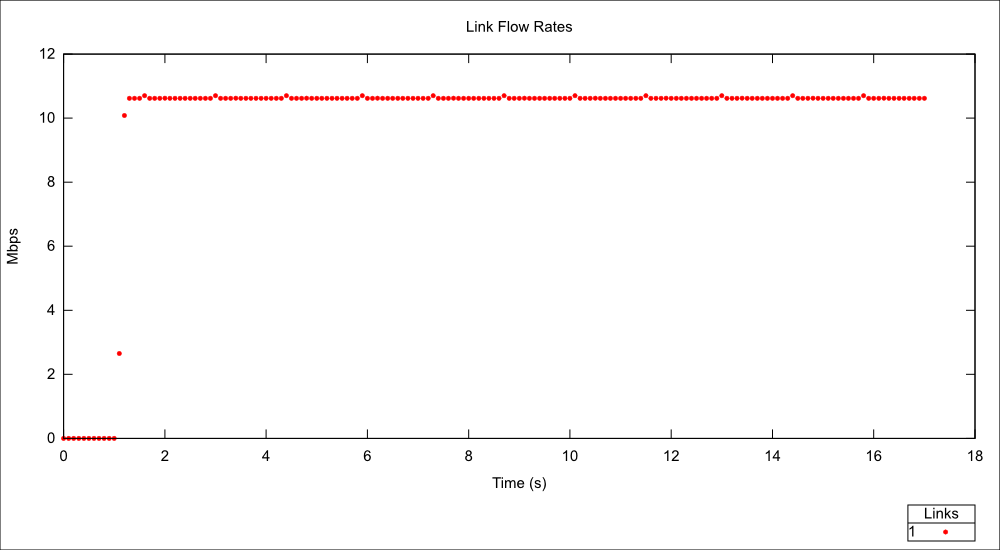
\includegraphics[width=\textwidth]{vegas0/Link_Flow_Rate.png}
    \caption{TCP VEGAS, Case 0: Host Send Rate}
\end{figure}

\begin{figure}[htbp]
    \centering
    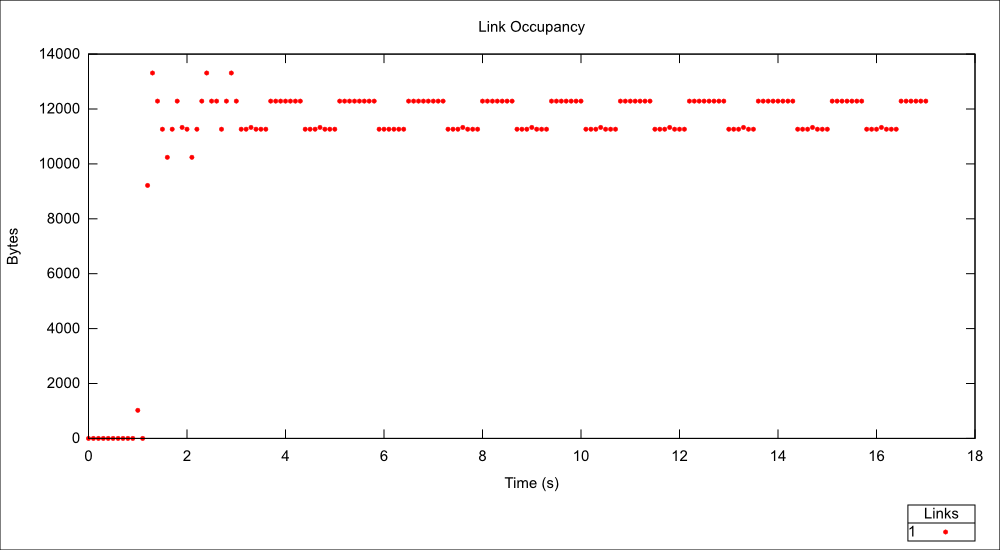
\includegraphics[width=\textwidth]{vegas0/Link_Occupancy.png}
    \caption{TCP VEGAS, Case 0: Host Send Rate}
\end{figure}

\begin{figure}[htbp]
    \centering
    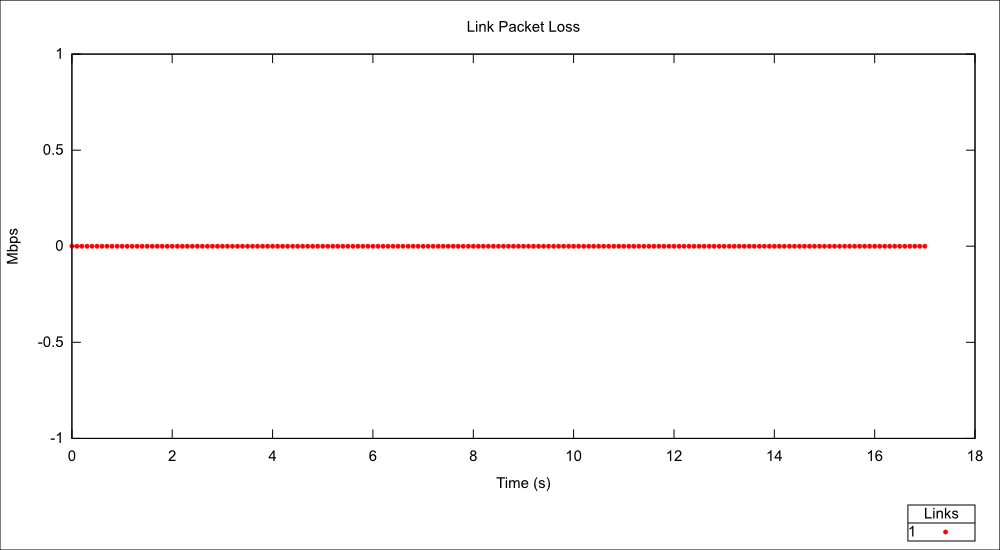
\includegraphics[width=\textwidth]{vegas0/Link_Packet_Loss.png}
    \caption{TCP VEGAS, Case 0: Host Send Rate}
\end{figure}

\newpage
\clearpage

%%%%%%%%%%%%%%%%%%%%%%%%%%%%%%%%%%%%%%%%%%%%%%%%%%%%%%%%%%%%%%%%%%%

\begin{figure}[htbp]
    \centering
    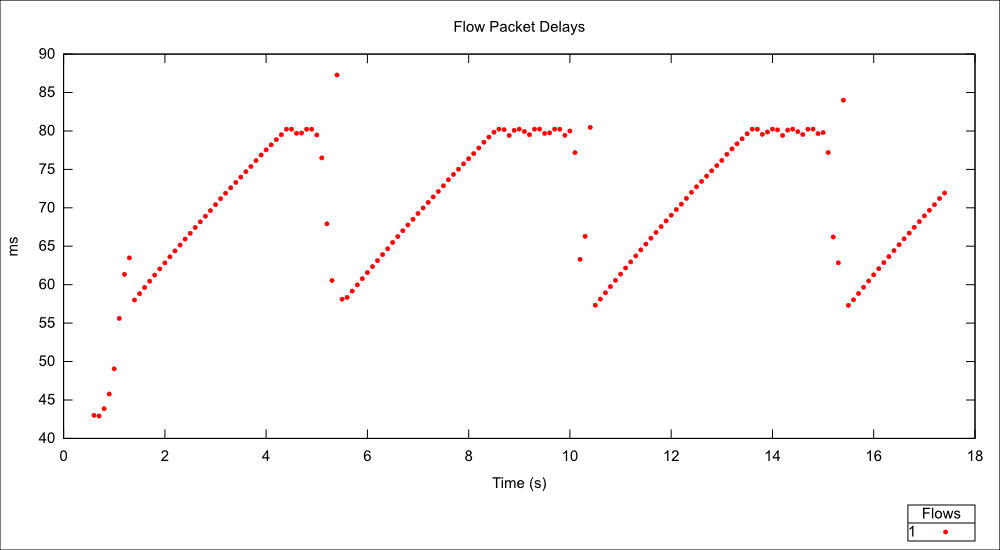
\includegraphics[width=\textwidth]{vegas1/Flow_RTT.png}
    \caption{TCP VEGAS, Case 1: Flow Round Trip Time}
\end{figure}

\begin{figure}[htbp]
    \centering
    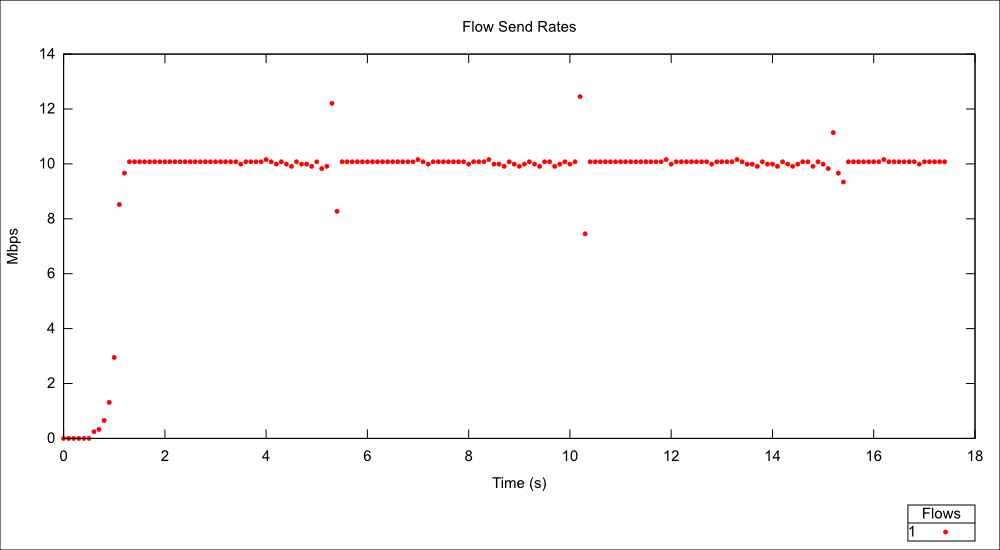
\includegraphics[width=\textwidth]{vegas1/Flow_Send_Rates.png}
    \caption{TCP VEGAS, Case 1: Flow Send Rates}
\end{figure}

\begin{figure}[htbp]
    \centering
    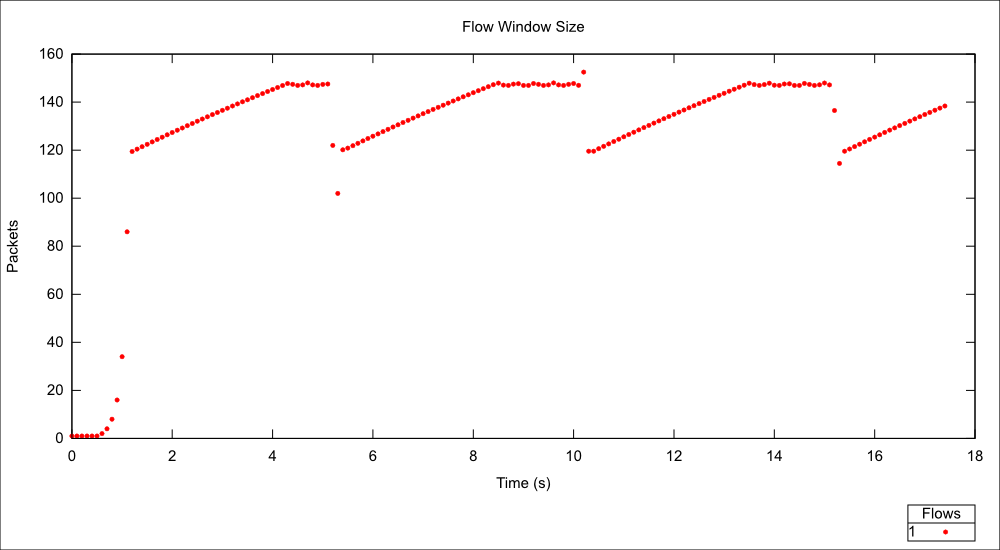
\includegraphics[width=\textwidth]{vegas1/Flow_Window.png}
    \caption{TCP VEGAS, Case 1: Flow Window}
\end{figure}


\begin{figure}[htbp]
    \centering
    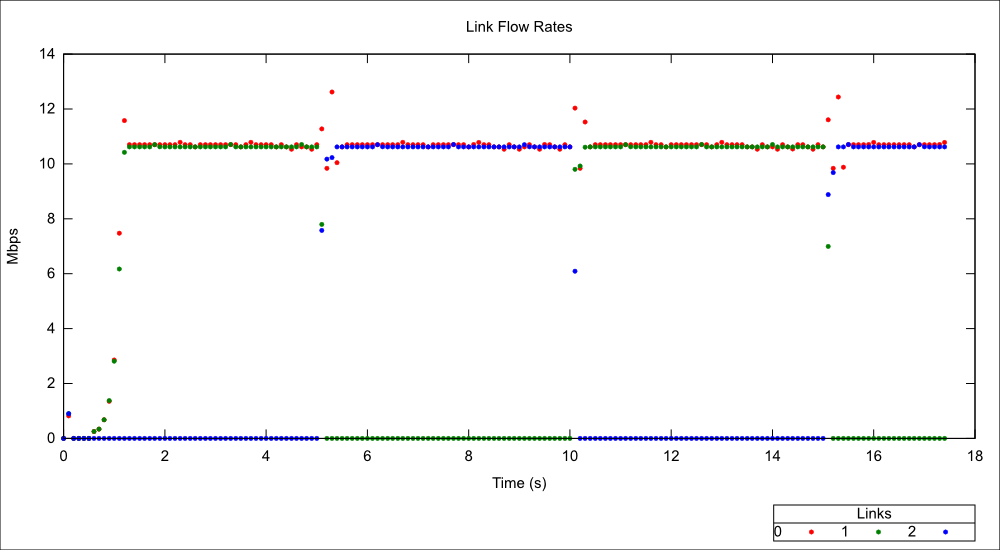
\includegraphics[width=\textwidth]{vegas1/Link_Flow_Rate.png}
    \caption{TCP VEGAS, Case 1: Host Send Rate}
\end{figure}

\begin{figure}[htbp]
    \centering
    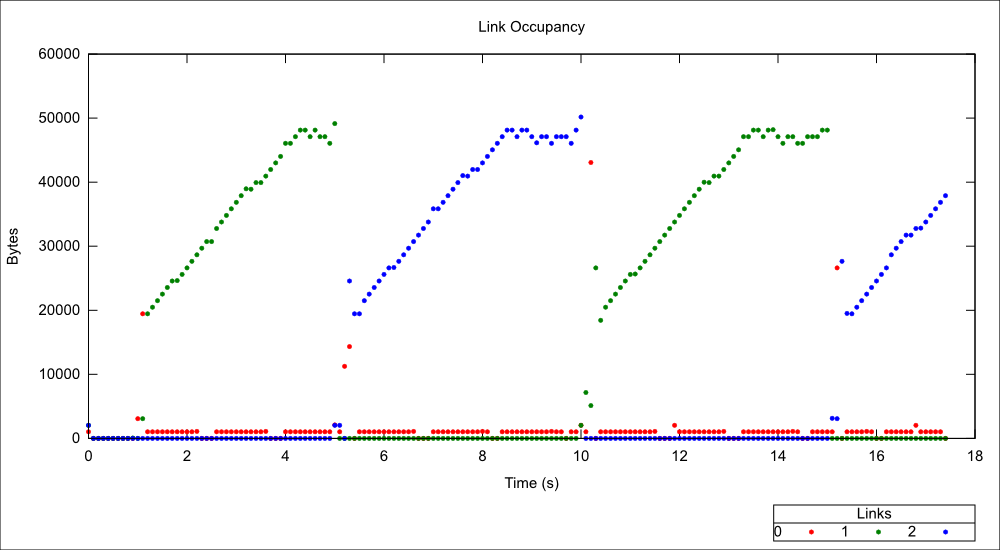
\includegraphics[width=\textwidth]{vegas1/Link_Occupancy.png}
    \caption{TCP VEGAS, Case 1: Host Send Rate}
\end{figure}

\begin{figure}[htbp]
    \centering
    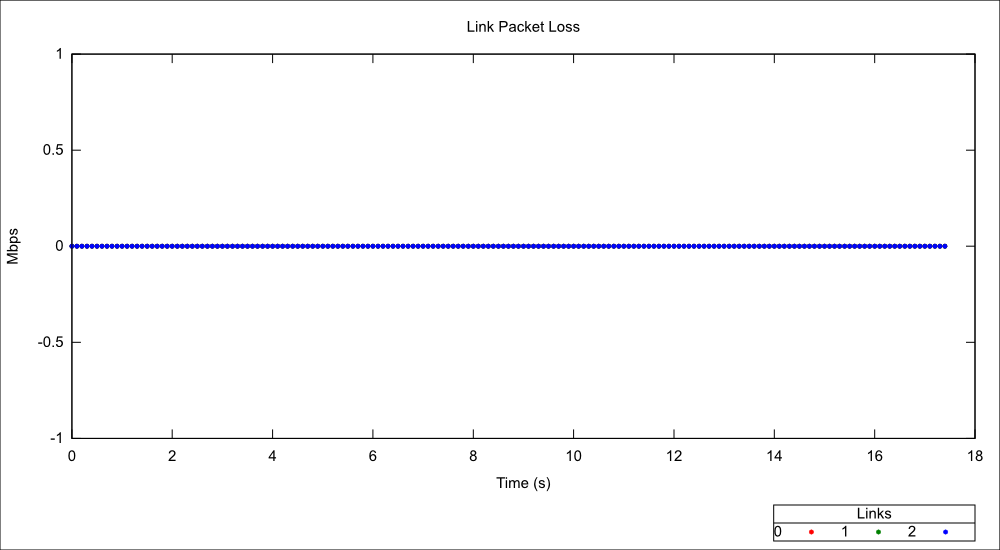
\includegraphics[width=\textwidth]{vegas1/Link_Packet_Loss.png}
    \caption{TCP VEGAS, Case 1: Host Send Rate}
\end{figure}

\newpage
\clearpage

%%%%%%%%%%%%%%%%%%%%%%%%%%%%%%%%%%%%%%%%%%%%%%%%%%%%%%%%%%%%%%%%%%%

\begin{figure}[htbp]
    \centering
    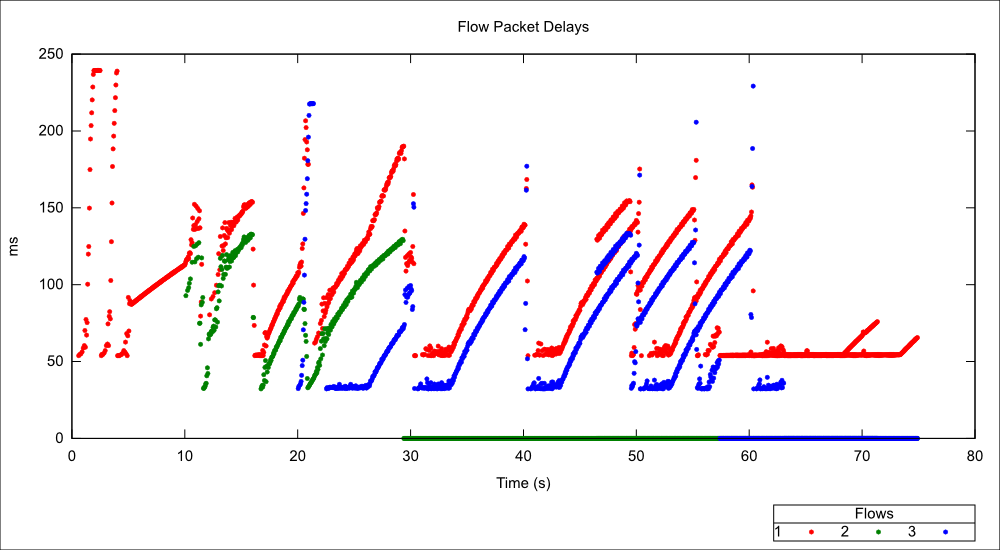
\includegraphics[width=\textwidth]{vegas2/Flow_RTT.png}
    \caption{TCP VEGAS, Case 2: Flow Round Trip Time}
\end{figure}

\begin{figure}[htbp]
    \centering
    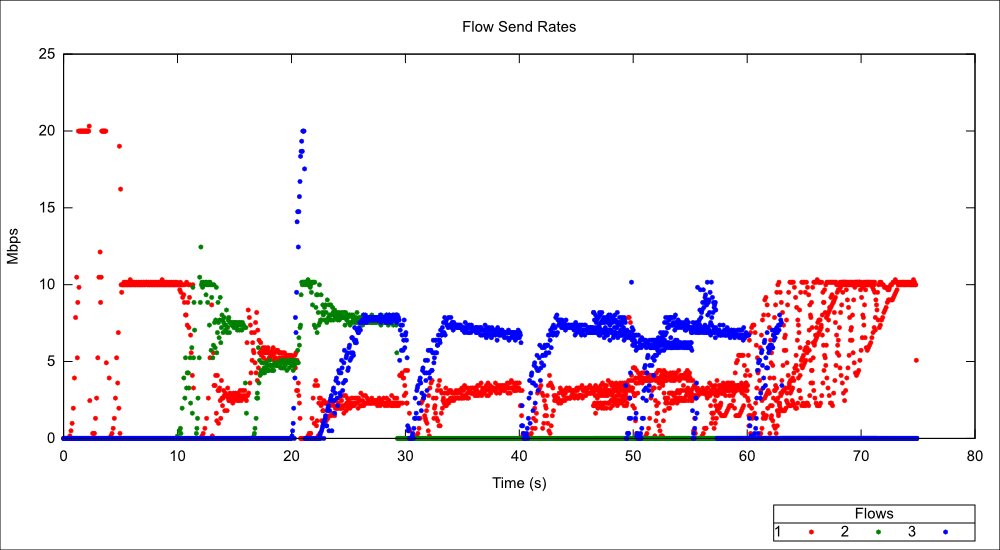
\includegraphics[width=\textwidth]{vegas2/Flow_Send_Rates.png}
    \caption{TCP VEGAS, Case 2: Flow Send Rates}
\end{figure}

\begin{figure}[htbp]
    \centering
    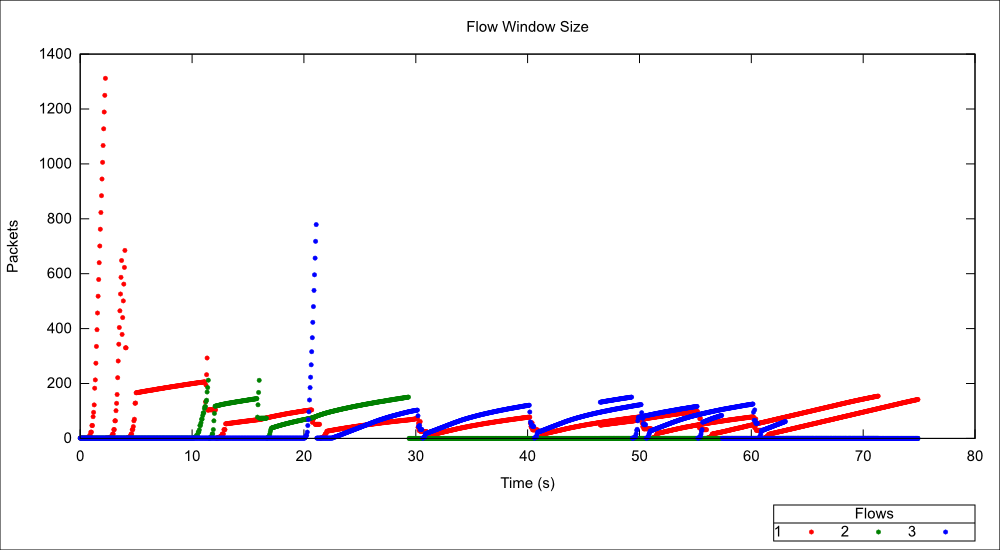
\includegraphics[width=\textwidth]{vegas2/Flow_Window.png}
    \caption{TCP VEGAS, Case 2: Flow Window}
\end{figure}


\begin{figure}[htbp]
    \centering
    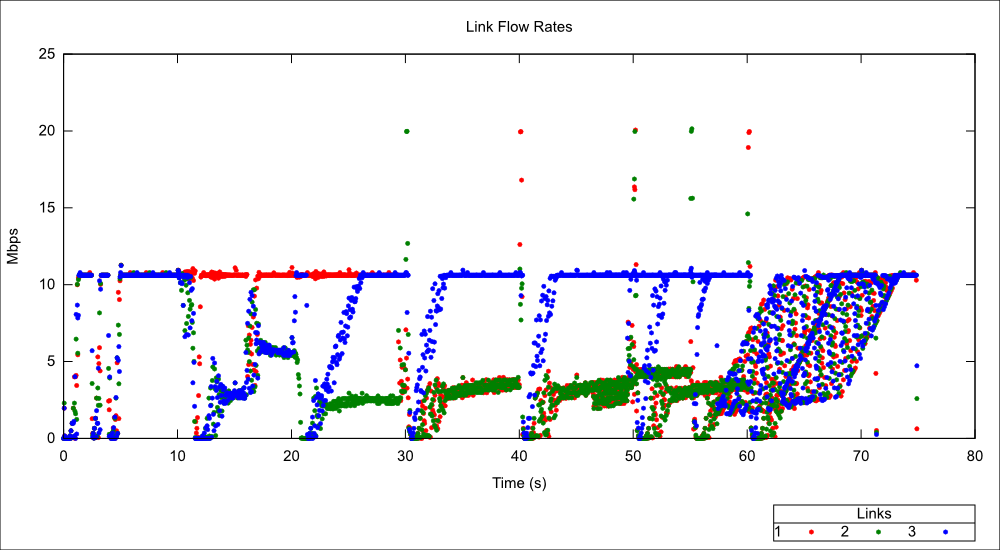
\includegraphics[width=\textwidth]{vegas2/Link_Flow_Rate.png}
    \caption{TCP VEGAS, Case 2: Host Send Rate}
\end{figure}

\begin{figure}[htbp]
    \centering
    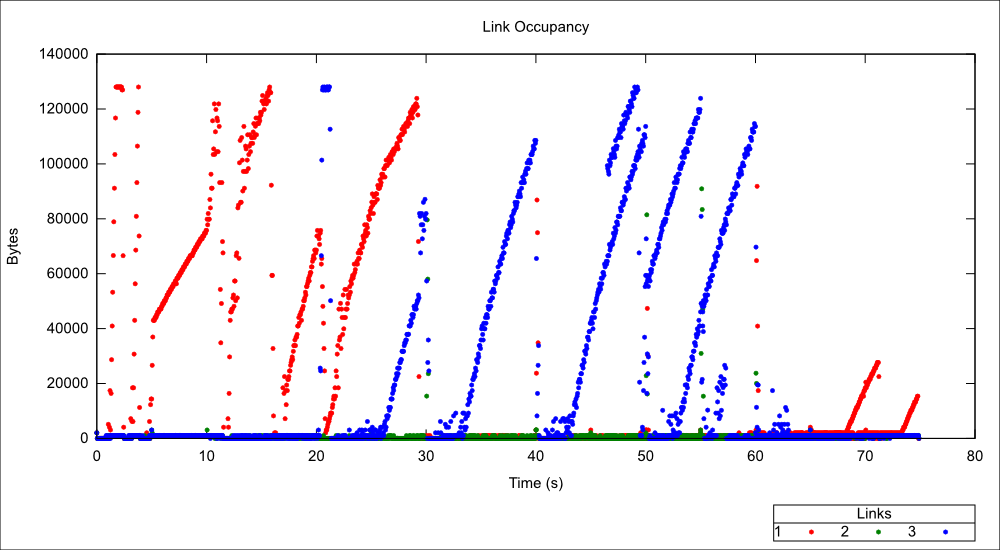
\includegraphics[width=\textwidth]{vegas2/Link_Occupancy.png}
    \caption{TCP VEGAS, Case 2: Host Send Rate}
\end{figure}

\begin{figure}[htbp]
    \centering
    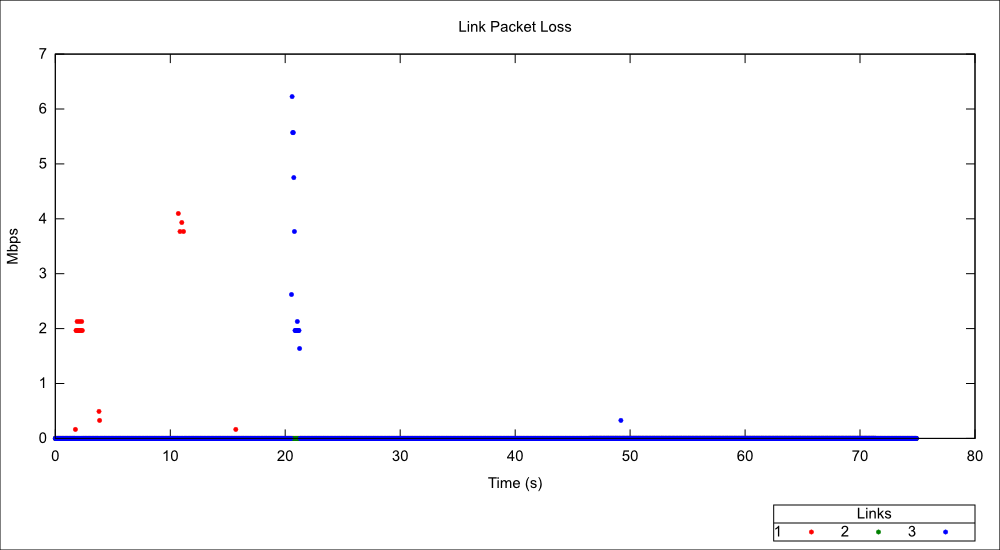
\includegraphics[width=\textwidth]{vegas2/Link_Packet_Loss.png}
    \caption{TCP VEGAS, Case 2: Host Send Rate}
\end{figure}

\newpage
\clearpage

%%%%%%%%%%%%%%%%%%%%%%%%%%%%%%%%%%%%%%%%%%%%%%%%%%%%%%%%%%%%%%%%%%%

\begin{figure}[htbp]
    \centering
    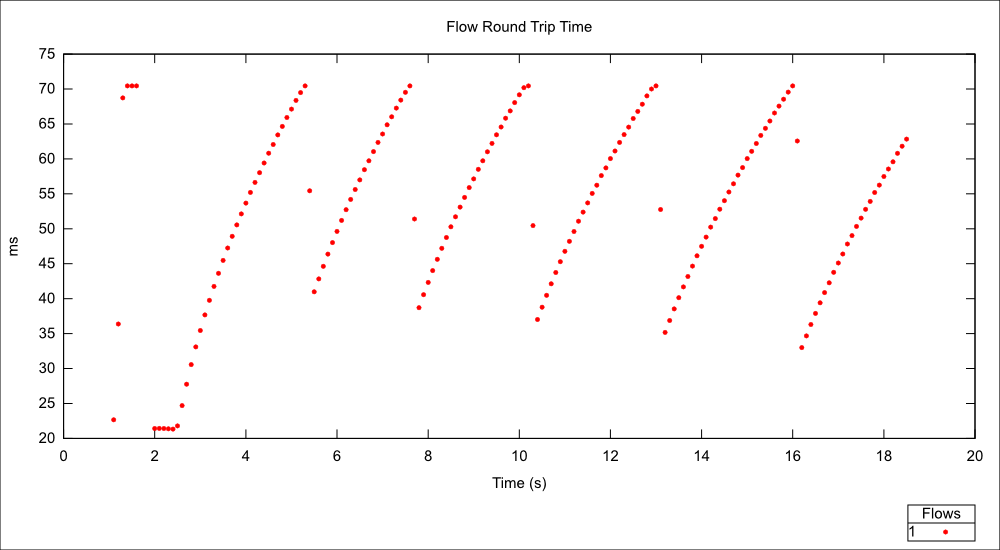
\includegraphics[width=\textwidth]{reno0/Flow_RTT.png}
    \caption{TCP RENO, Case 0: Flow Round Trip Time}
\end{figure}

\begin{figure}[htbp]
    \centering
    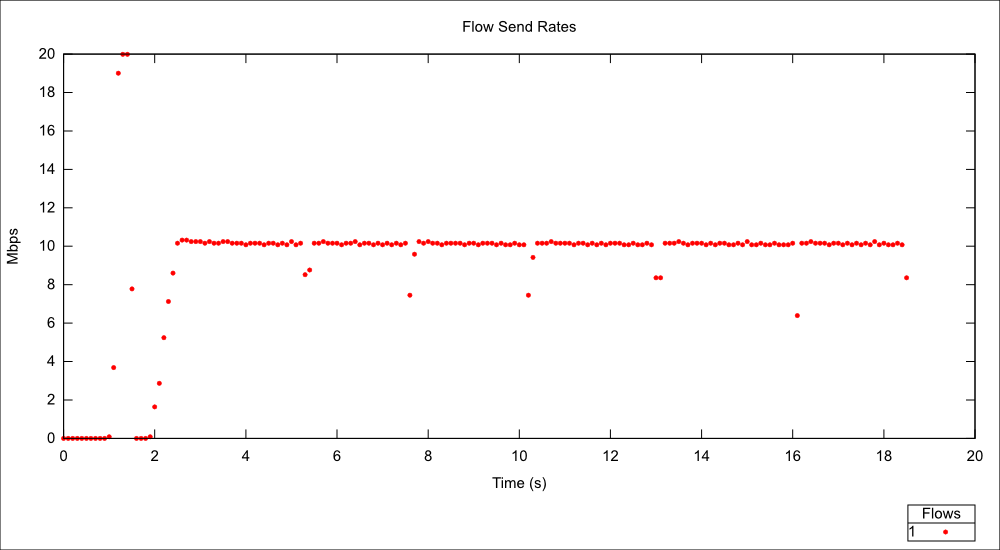
\includegraphics[width=\textwidth]{reno0/Flow_Send_Rates.png}
    \caption{TCP RENO, Case 0: Flow Send Rates}
\end{figure}

\begin{figure}[htbp]
    \centering
    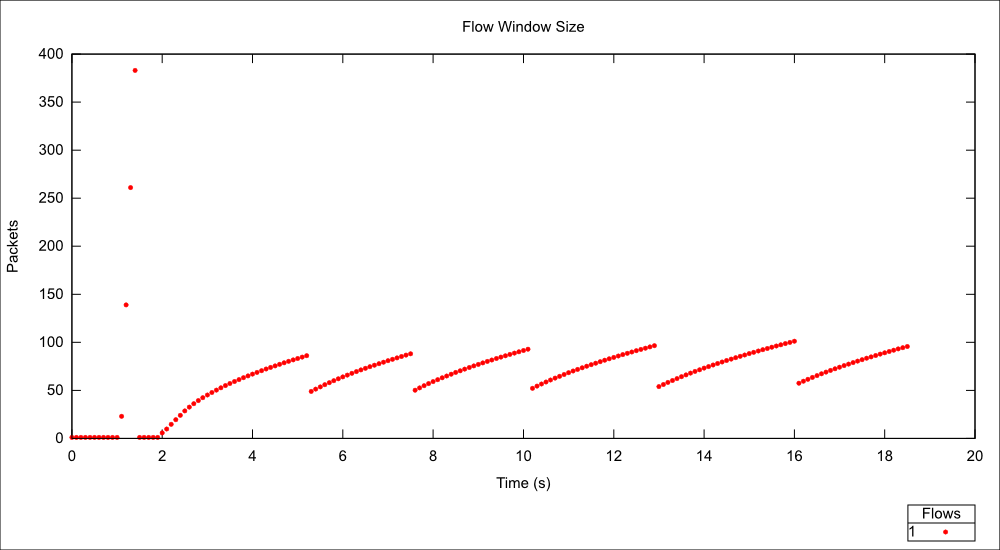
\includegraphics[width=\textwidth]{reno0/Flow_Window.png}
    \caption{TCP RENO, Case 0: Flow Window}
\end{figure}


\begin{figure}[htbp]
    \centering
    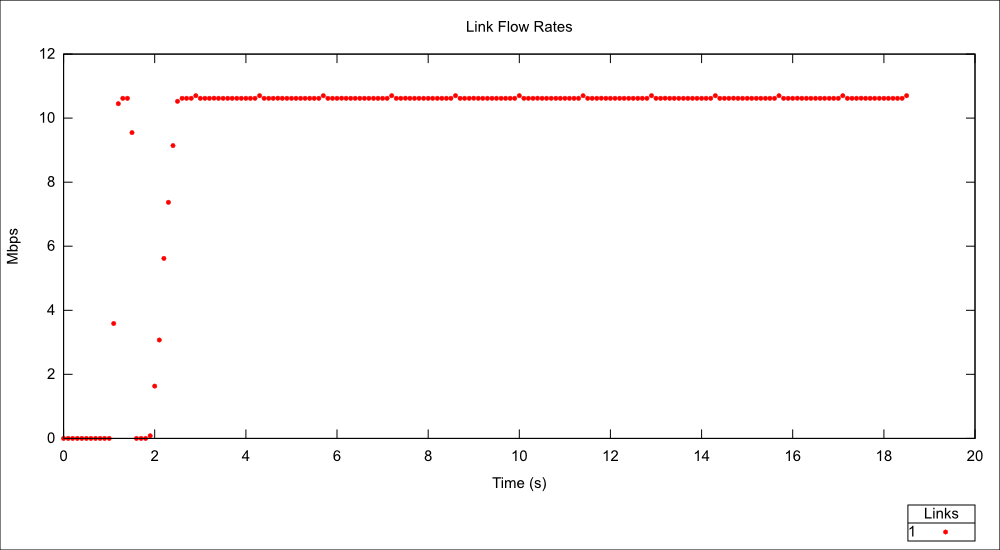
\includegraphics[width=\textwidth]{reno0/Link_Flow_Rate.png}
    \caption{TCP RENO, Case 0: Host Send Rate}
\end{figure}

\begin{figure}[htbp]
    \centering
    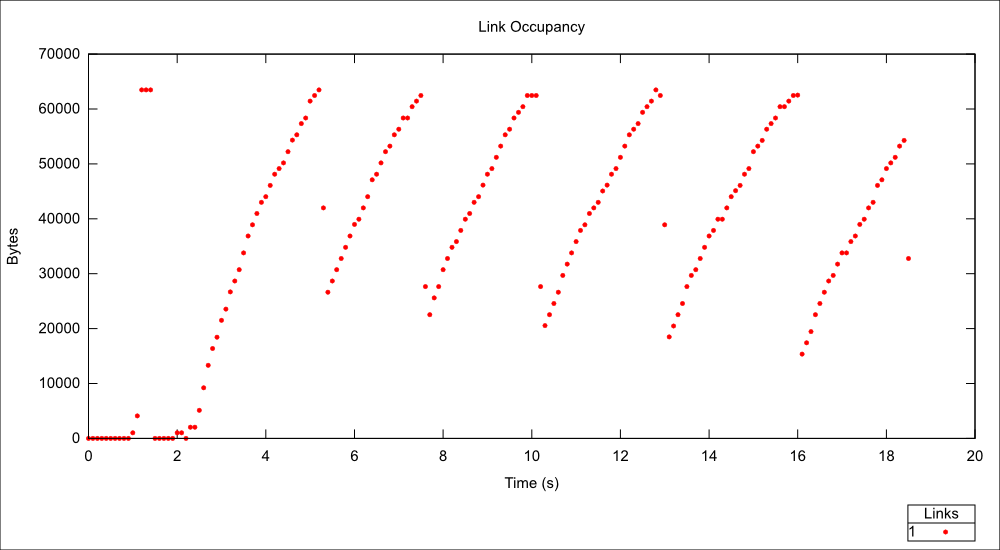
\includegraphics[width=\textwidth]{reno0/Link_Occupancy.png}
    \caption{TCP RENO, Case 0: Host Send Rate}
\end{figure}

\begin{figure}[htbp]
    \centering
    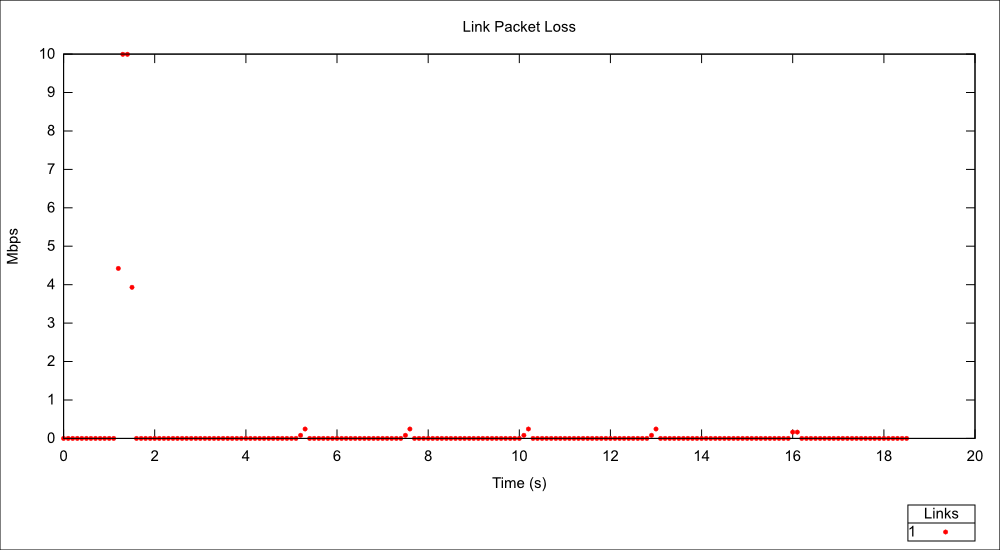
\includegraphics[width=\textwidth]{reno0/Link_Packet_Loss.png}
    \caption{TCP RENO, Case 0: Host Send Rate}
\end{figure}

\newpage
\clearpage

%%%%%%%%%%%%%%%%%%%%%%%%%%%%%%%%%%%%%%%%%%%%%%%%%%%%%%%%%%%%%%%%%%%

\begin{figure}[htbp]
    \centering
    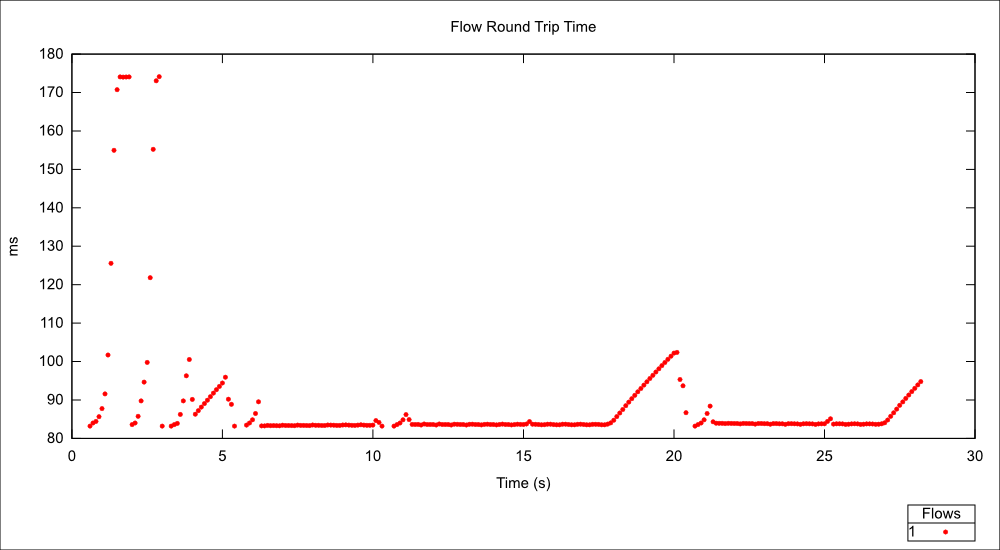
\includegraphics[width=\textwidth]{reno1/Flow_RTT.png}
    \caption{TCP RENO, Case 1: Flow Round Trip Time}
\end{figure}

\begin{figure}[htbp]
    \centering
    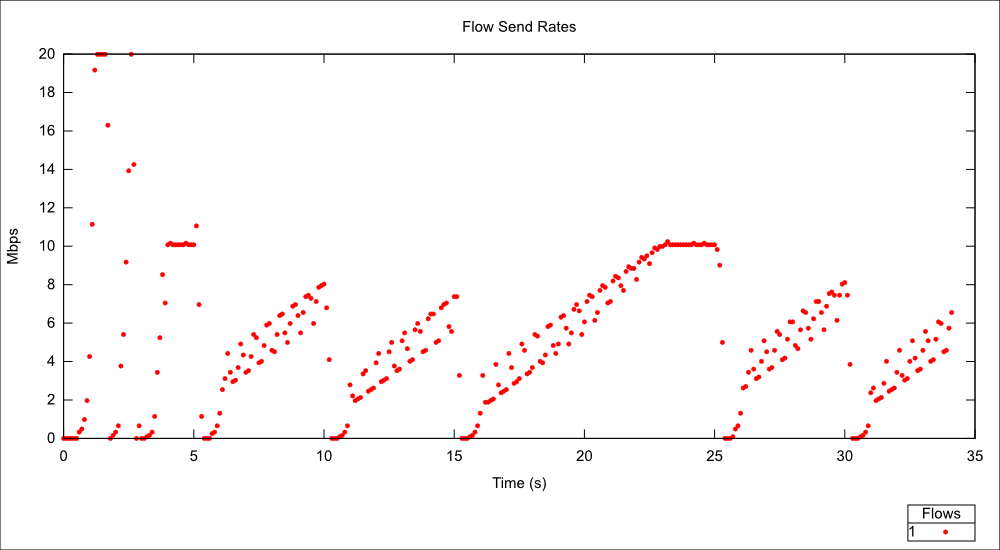
\includegraphics[width=\textwidth]{reno1/Flow_Send_Rates.png}
    \caption{TCP RENO, Case 1: Flow Send Rates}
\end{figure}

\begin{figure}[htbp]
    \centering
    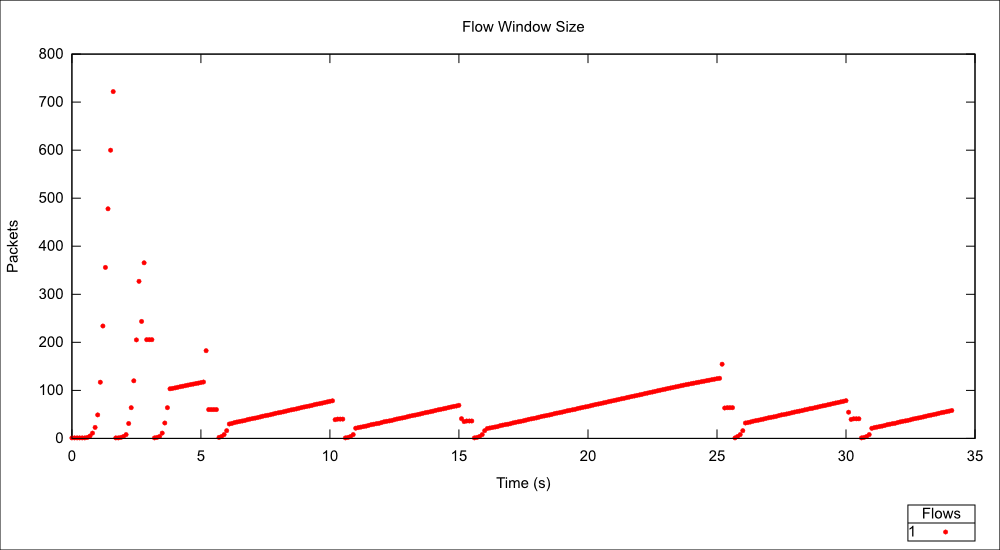
\includegraphics[width=\textwidth]{reno1/Flow_Window.png}
    \caption{TCP RENO, Case 1: Flow Window}
\end{figure}


\begin{figure}[htbp]
    \centering
    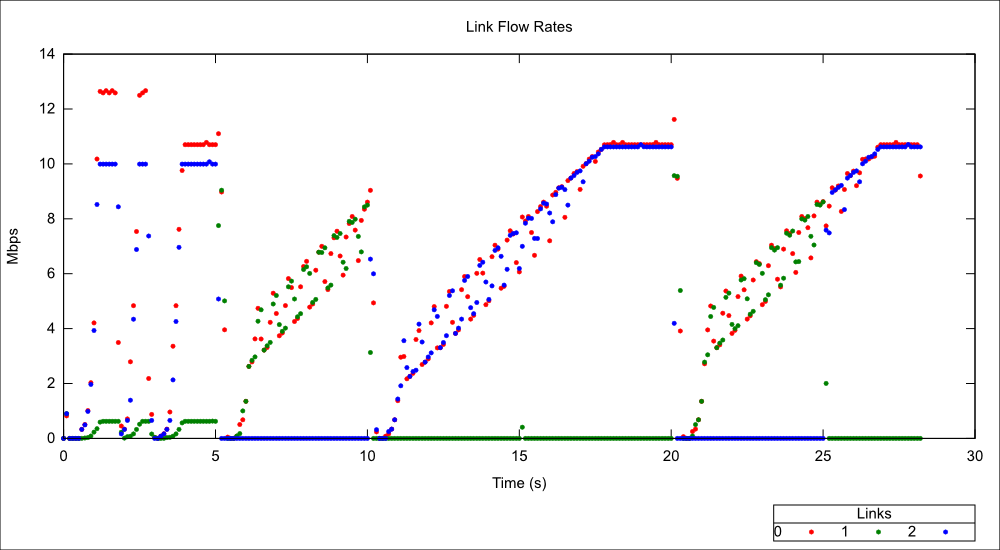
\includegraphics[width=\textwidth]{reno1/Link_Flow_Rate.png}
    \caption{TCP RENO, Case 1: Host Send Rate}
\end{figure}

\begin{figure}[htbp]
    \centering
    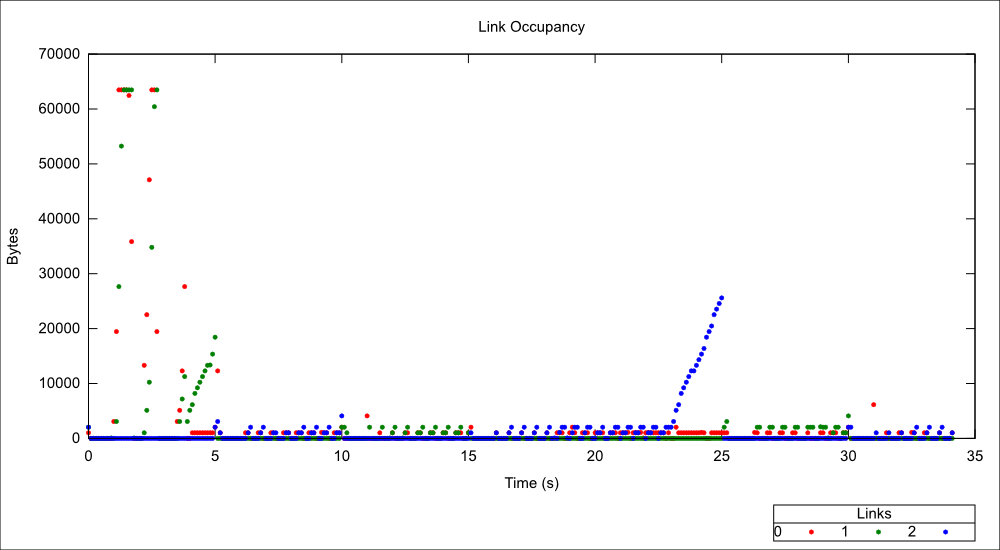
\includegraphics[width=\textwidth]{reno1/Link_Occupancy.png}
    \caption{TCP RENO, Case 1: Host Send Rate}
\end{figure}

\begin{figure}[htbp]
    \centering
    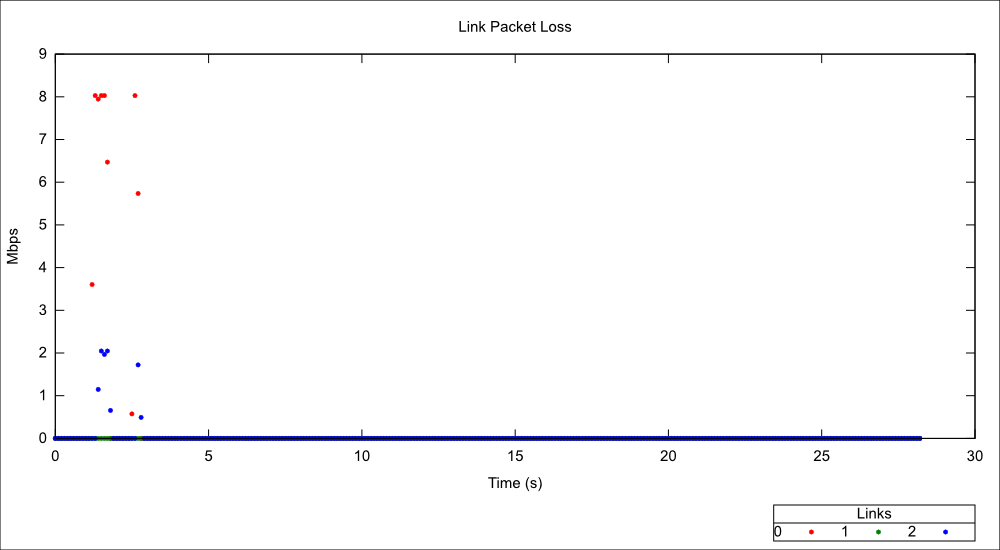
\includegraphics[width=\textwidth]{reno1/Link_Packet_Loss.png}
    \caption{TCP RENO, Case 1: Host Send Rate}
\end{figure}

\newpage
\clearpage

%%%%%%%%%%%%%%%%%%%%%%%%%%%%%%%%%%%%%%%%%%%%%%%%%%%%%%%%%%%%%%%%%%%

\begin{figure}[htbp]
    \centering
    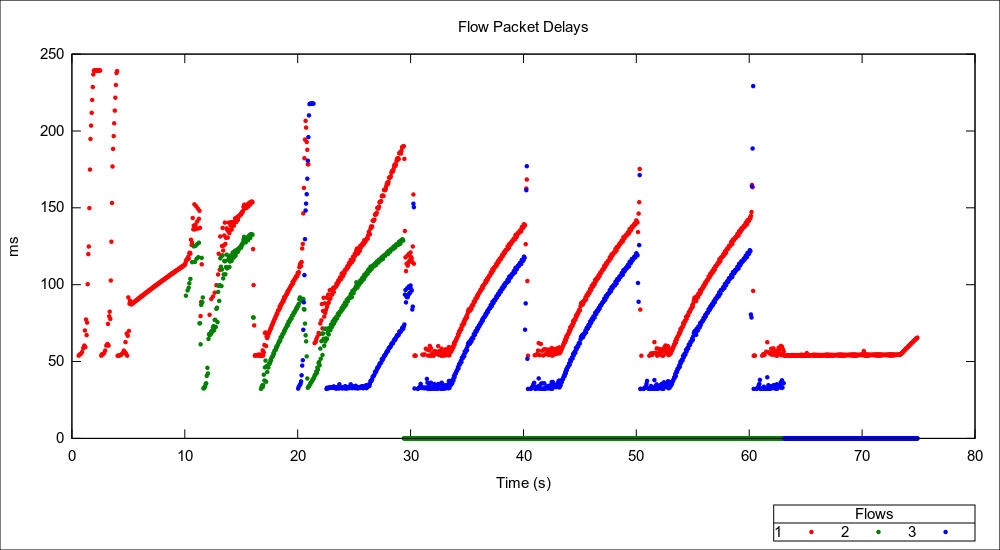
\includegraphics[width=\textwidth]{reno2/Flow_RTT.png}
    \caption{TCP RENO, Case 2: Flow Round Trip Time}
\end{figure}

\begin{figure}[htbp]
    \centering
    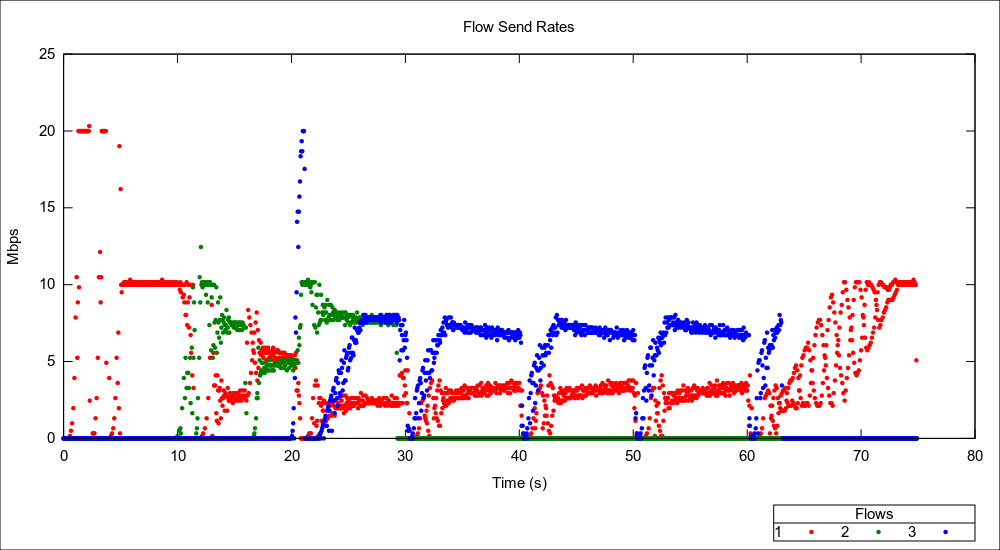
\includegraphics[width=\textwidth]{reno2/Flow_Send_Rates.png}
    \caption{TCP RENO, Case 2: Flow Send Rates}
\end{figure}

\begin{figure}[htbp]
    \centering
    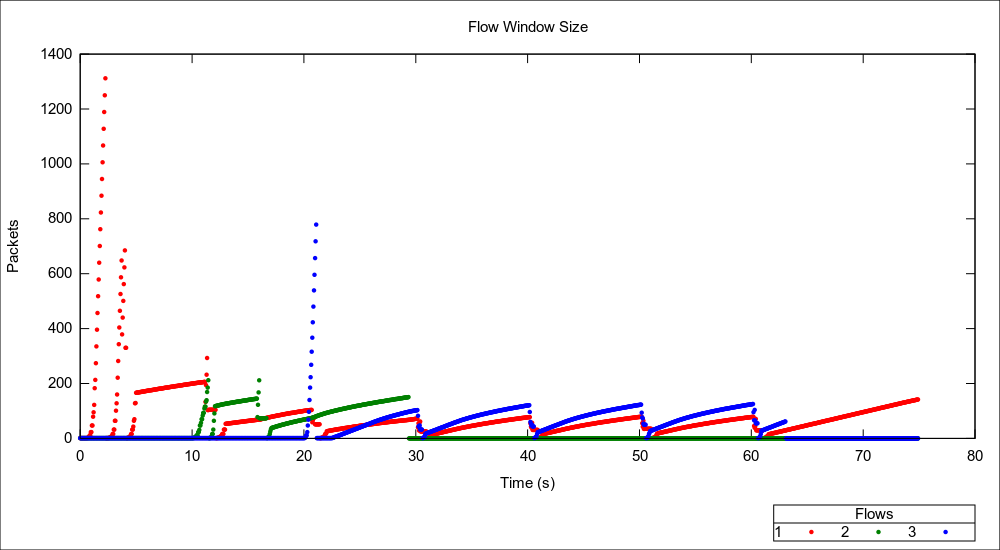
\includegraphics[width=\textwidth]{reno2/Flow_Window.png}
    \caption{TCP RENO, Case 2: Flow Window}
\end{figure}


\begin{figure}[htbp]
    \centering
    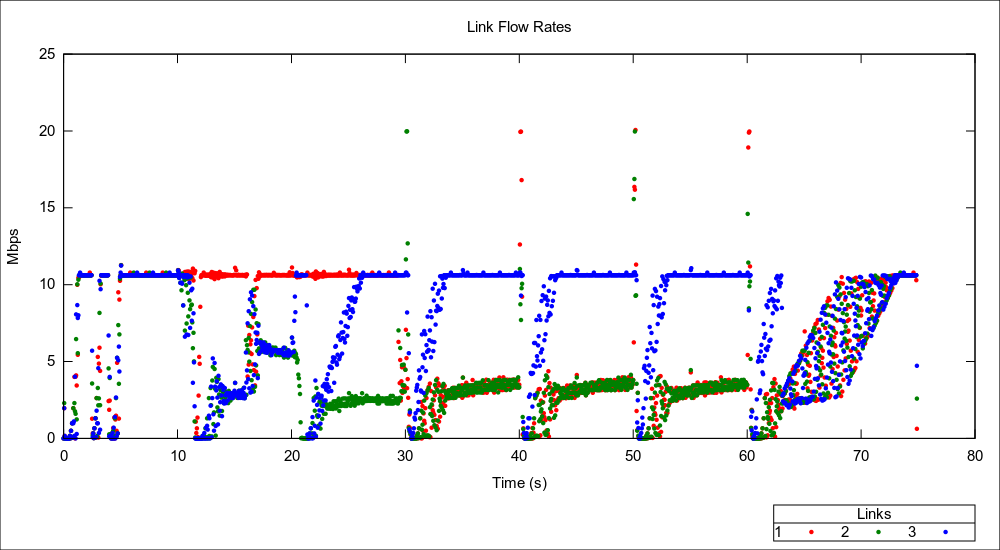
\includegraphics[width=\textwidth]{reno2/Link_Flow_Rate.png}
    \caption{TCP RENO, Case 2: Host Send Rate}
\end{figure}

\begin{figure}[htbp]
    \centering
    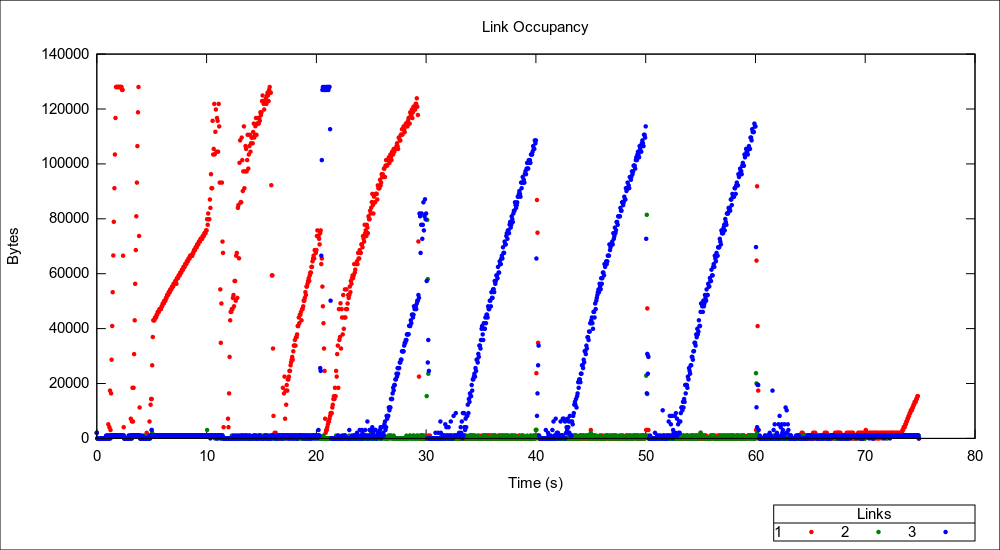
\includegraphics[width=\textwidth]{reno2/Link_Occupancy.png}
    \caption{TCP RENO, Case 2: Host Send Rate}
\end{figure}

\begin{figure}[htbp]
    \centering
    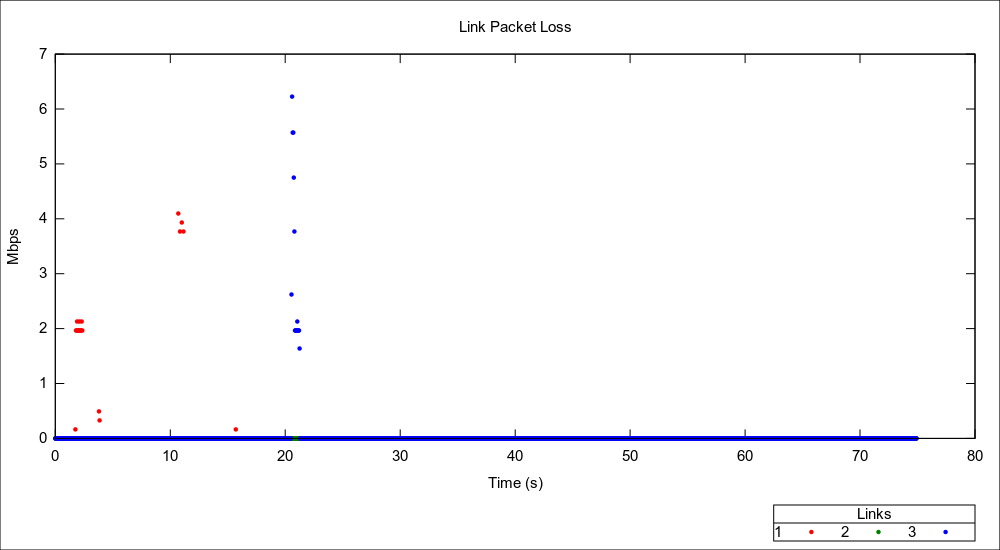
\includegraphics[width=\textwidth]{reno2/Link_Packet_Loss.png}
    \caption{TCP RENO, Case 2: Host Send Rate}
\end{figure}

\newpage
\clearpage

